\section{USB CDC Protocol}
\label{sec:usb_cdc_protocol}

\subsection{Overview}

The RX72N firmware implements a USB CDC-ACM (Communications Device Class - Abstract Control Model) composite device with three independent virtual serial ports. This enables simultaneous binary protocol communication, ASCII debugging, and log streaming over a single USB connection.

\subsubsection{Port Assignment}

\begin{table}[h]
\centering
\begin{tabular}{|c|l|l|c|c|p{4cm}|}
\hline
\textbf{Port} & \textbf{Purpose} & \textbf{Linux Device} & \textbf{RX (B)} & \textbf{TX (B)} & \textbf{Usage} \\
\hline
0 & Protocol & /dev/ttyACM0 & 1024 & 1024 & nanopb frames, motor commands \\
1 & Decoded & /dev/ttyACM1 & 256 & 512 & ASCII frame dumps, debugging \\
2 & Log & /dev/ttyACM2 & 256 & 1024 & System logging, diagnostics \\
\hline
\end{tabular}
\caption{USB CDC Port Configuration}
\label{tab:usb_cdc_ports}
\end{table}

\subsubsection{Hardware Configuration}

\begin{itemize}
\item \textbf{USB Speed}: Full-Speed (12 Mbps)
\item \textbf{Max Packet Size}: 64 bytes (bulk endpoints)
\item \textbf{Pipes Used}: 9 pipes total (1 control + 3 CDC × (1 interrupt + 2 bulk))
\item \textbf{Pins}: USB\_DP (PA4), USB\_DM (PA5), USB\_VBUS (PA6)
\item \textbf{Clock}: 48 MHz USB clock from PLL
\end{itemize}

\subsection{USB Descriptor Hierarchy}

\subsubsection{Device Descriptor}

\begin{lstlisting}[language=C,caption={USB Device Descriptor},label={lst:usb_device_desc}]
{
  .bLength = 18,
  .bDescriptorType = USB_DEVICE_DESCRIPTOR,
  .bcdUSB = 0x0200,              // USB 2.0
  .bDeviceClass = 0xEF,          // Miscellaneous (IAD)
  .bDeviceSubClass = 0x02,       // Common Class
  .bDeviceProtocol = 0x01,       // Interface Association
  .bMaxPacketSize0 = 64,
  .idVendor = 0x045B,            // Renesas
  .idProduct = 0x024F,           // RX72N CDC
  .bcdDevice = 0x0100,           // Device v1.0
  .iManufacturer = 1,            // "STAR Project"
  .iProduct = 2,                 // "RX72N CDC Composite"
  .iSerialNumber = 3,            // "RX72N-00001"
  .bNumConfigurations = 1
}
\end{lstlisting}

\subsubsection{Configuration Descriptor}

The configuration descriptor contains:
\begin{itemize}
\item 3 × Interface Association Descriptors (IAD) - Groups each CDC function
\item 3 × CDC Control Interface (Class 0x02, Subclass 0x02)
\item 3 × CDC Data Interface (Class 0x0A, Subclass 0x00)
\item 3 × Interrupt IN endpoints (control)
\item 6 × Bulk endpoints (3 IN + 3 OUT for data)
\end{itemize}

\subsubsection{Interface Association Descriptor (IAD)}

Each CDC port uses an IAD to group its control and data interfaces:

\begin{lstlisting}[language=C,caption={IAD for Port 0 (Protocol Port)},label={lst:usb_iad}]
{
  .bLength = 8,
  .bDescriptorType = 0x0B,       // IAD
  .bFirstInterface = 0,          // Control interface
  .bInterfaceCount = 2,          // Control + Data
  .bFunctionClass = 0x02,        // CDC
  .bFunctionSubClass = 0x02,     // ACM
  .bFunctionProtocol = 0x01,     // AT Commands
  .iFunction = 4                 // "Protocol Port"
}
\end{lstlisting}

\subsubsection{Endpoint Configuration}

\begin{table}[h]
\centering
\begin{tabular}{|c|l|c|c|c|c|}
\hline
\textbf{Port} & \textbf{Type} & \textbf{EP} & \textbf{Dir} & \textbf{Size} & \textbf{Interval} \\
\hline
0 & Interrupt & EP1 & IN & 16 & 10 ms \\
0 & Bulk OUT & EP2 & OUT & 64 & - \\
0 & Bulk IN & EP3 & IN & 64 & - \\
\hline
1 & Interrupt & EP4 & IN & 16 & 10 ms \\
1 & Bulk OUT & EP5 & OUT & 64 & - \\
1 & Bulk IN & EP6 & IN & 64 & - \\
\hline
2 & Interrupt & EP7 & IN & 16 & 10 ms \\
2 & Bulk OUT & EP8 & OUT & 64 & - \\
2 & Bulk IN & EP9 & IN & 64 & - \\
\hline
\end{tabular}
\caption{USB Endpoint Assignments}
\label{tab:usb_endpoints}
\end{table}

\subsection{USB State Machine}

\begin{figure}[h]
\centering
\begin{tikzpicture}[node distance=2cm, auto]
  \node[state] (detached) {Detached};
  \node[state, right of=detached] (attached) {Attached};
  \node[state, right of=attached] (powered) {Powered};
  \node[state, below of=powered] (default) {Default};
  \node[state, left of=default] (addressed) {Addressed};
  \node[state, left of=addressed] (configured) {Configured};
  \node[state, below of=configured] (suspended) {Suspended};

  \path[->]
    (detached) edge node {VBUS detect} (attached)
    (attached) edge node {auto} (powered)
    (powered) edge node {Bus Reset} (default)
    (default) edge node {SET\_ADDRESS} (addressed)
    (addressed) edge node {SET\_CONFIG} (configured)
    (configured) edge node {3ms idle} (suspended)
    (suspended) edge[bend right] node {Resume} (configured)
    (configured) edge[bend right=60] node[below] {VBUS lost} (detached)
    (default) edge[bend left=40] node {Bus Reset} (default);
\end{tikzpicture}
\caption{USB Device State Machine}
\label{fig:usb_state_machine}
\end{figure}

\textbf{Critical State}: Only in \texttt{Configured} state can \texttt{rx\_usb\_write/read} transfer data.

\subsection{CDC-ACM Class Requests}

The USB CDC driver handles these class-specific requests:

\begin{table}[h]
\centering
\begin{tabular}{|l|c|p{6cm}|}
\hline
\textbf{Request} & \textbf{Code} & \textbf{Description} \\
\hline
SET\_LINE\_CODING & 0x20 & Host configures baud rate, parity, stop bits \\
GET\_LINE\_CODING & 0x21 & Host queries current line coding \\
SET\_CONTROL\_LINE\_STATE & 0x22 & DTR/RTS control signals (ignored) \\
\hline
\end{tabular}
\caption{CDC-ACM Class Requests}
\label{tab:cdc_requests}
\end{table}

\textbf{Note}: Line coding settings (baud rate, parity, etc.) are informational only. USB CDC operates at USB Full-Speed (12 Mbps), not the configured baud rate.

\subsection{Bulk Transfer Protocol}

\subsubsection{Data Flow}

\paragraph{Bulk OUT (Host → Device)}

\begin{enumerate}
\item Host writes data to /dev/ttyACM*
\item USB driver sends bulk OUT packet (max 64 bytes)
\item RX72N receives packet → BRDY interrupt fires
\item ISR reads FIFO → copies to RX ring buffer
\item Application calls \texttt{rx\_usb\_read()} → retrieves data
\end{enumerate}

\paragraph{Bulk IN (Device → Host)}

\begin{enumerate}
\item Application calls \texttt{rx\_usb\_write()} → copies to TX ring buffer
\item ISR writes FIFO → sends bulk IN packet (max 64 bytes)
\item BEMP interrupt fires when packet sent
\item Host reads data from /dev/ttyACM*
\end{enumerate}

\subsubsection{FIFO Access Requirements (RX72N-Specific)}

\textbf{CRITICAL}: RX72N USB FIFO registers \textbf{must} be accessed as 16-bit words, NOT byte-by-byte.

\begin{lstlisting}[language=C,caption={Correct FIFO Read (16-bit access)},label={lst:fifo_read_correct}]
// CORRECT: Read CFIFO as 16-bit words
for (uint32_t i = 0; i < len; i += 2) {
  const uint16_t word = usb0()->cfifo;  // 16-bit read
  data[i] = (uint8_t)(word & 0xFF);     // Low byte
  if ((i + 1) < len) {
    data[i + 1] = (uint8_t)((word >> 8) & 0xFF);  // High byte
  }
}
\end{lstlisting}

\begin{lstlisting}[language=C,caption={Incorrect FIFO Read (causes data corruption)},label={lst:fifo_read_wrong}]
// WRONG: Byte-by-byte access causes corruption
for (uint32_t i = 0; i < len; i++) {
  data[i] = (uint8_t)(usb0()->cfifo & 0xFF);  // BAD!
}
\end{lstlisting}

\textbf{Impact}: Byte-by-byte access was the root cause of all bulk transfer failures before Phase 2 fixes.

\subsubsection{FIFO Clear Sequence}

Before writing to FIFO, the BCLR (Buffer Clear) sequence must be executed:

\begin{lstlisting}[language=C,caption={FIFO Clear Before Write},label={lst:fifo_clear}]
// Set BCLR bit (hardware clears FIFO)
usb0()->cfifoctr |= k_usb_fifoctr_bclr;

// Wait for BCLR to complete (hardware clears bit)
uint32_t timeout = 10000;
while ((usb0()->cfifoctr & k_usb_fifoctr_bclr) && timeout--) {
  __asm__ volatile("nop");
}

// Now safe to write data
for (uint32_t i = 0; i < len; i += 2) {
  // ... 16-bit write ...
}
\end{lstlisting}

\textbf{Impact}: Missing BCLR sequence caused first packet corruption with stale data.

\subsection{Debug Logging Over USB CDC Port 2}

\subsubsection{Architecture}

The logging system supports dual output to both UART and USB CDC Port 2:

\begin{itemize}
\item \textbf{UART (SCI12)}: Always works, independent of USB state
\item \textbf{USB CDC Port 2}: Enabled when \texttt{USB\_LOG\_MIRROR=1}
\item \textbf{Boot buffering}: 512B ring buffer for logs during USB enumeration (0-200ms)
\item \textbf{Thread safety}: ThreadX mutex for multi-task logging
\item \textbf{Non-blocking}: Drops logs on TX full, tracks statistics
\end{itemize}

\subsubsection{Boot Log Sequence}

\begin{figure}[h]
\centering
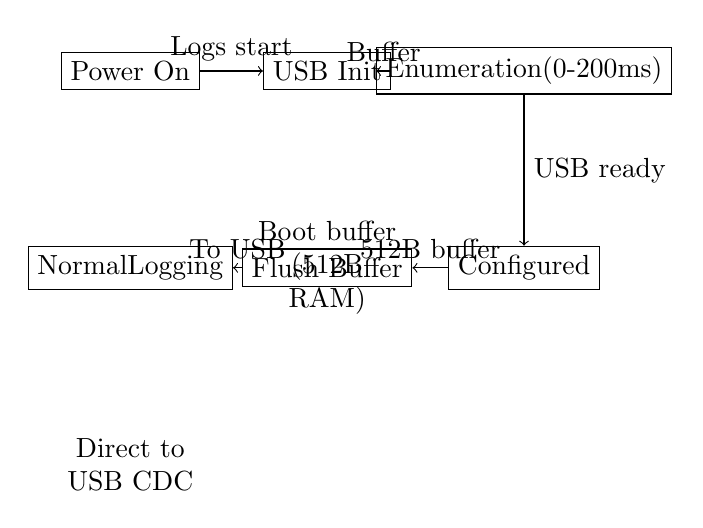
\begin{tikzpicture}[node distance=2.5cm, auto]
  \node[rectangle, draw] (power) {Power On};
  \node[rectangle, draw, right of=power] (usb_init) {USB Init};
  \node[rectangle, draw, right of=usb_init] (enum) {Enumeration\\(0-200ms)};
  \node[rectangle, draw, below of=enum] (configured) {Configured};
  \node[rectangle, draw, left of=configured] (flush) {Flush Buffer};
  \node[rectangle, draw, left of=flush] (normal) {Normal\\Logging};

  \draw[->] (power) -- node[above] {Logs start} (usb_init);
  \draw[->] (usb_init) -- node[above] {Buffer} (enum);
  \draw[->] (enum) -- node[right] {USB ready} (configured);
  \draw[->] (configured) -- node[above] {512B buffer} (flush);
  \draw[->] (flush) -- node[above] {To USB} (normal);

  \node[below of=usb_init, text width=2cm, align=center] {Boot buffer\\(512B RAM)};
  \node[below of=normal, text width=2cm, align=center] {Direct to\\USB CDC};
\end{tikzpicture}
\caption{Boot Log Buffering Sequence}
\label{fig:boot_log_sequence}
\end{figure}

\subsubsection{Implementation}

\paragraph{Boot Buffer Structure}

\begin{lstlisting}[language=C,caption={Boot Log Ring Buffer},label={lst:boot_buffer}]
typedef struct {
  char     data[512];    // Ring buffer storage
  uint16_t head;         // Write index
  uint16_t count;        // Buffered bytes
  bool     overflow;     // Overflow flag
} usb_log_boot_buffer_t;

static usb_log_boot_buffer_t s_boot_buffer = {0};
static volatile bool s_usb_ready = false;
\end{lstlisting}

\paragraph{Log Write Flow}

\begin{enumerate}
\item Application calls \texttt{rx\_log\_info()}, \texttt{rx\_log\_warn()}, etc.
\item Macro expands to \texttt{uart\_debug\_puts()} + \texttt{rx\_log\_usb\_puts()}
\item \texttt{rx\_log\_usb\_puts()} acquires ThreadX mutex
\item Check USB state:
  \begin{itemize}
  \item \textbf{Not configured}: Buffer to 512B ring buffer
  \item \textbf{Configured}: Write directly to USB CDC Port 2 via \texttt{rx\_usb\_write()}
  \end{itemize}
\item If USB TX buffer full (\texttt{k\_rx\_err\_busy}): Drop log, increment \texttt{dropped\_bytes}
\item Release mutex
\end{enumerate}

\paragraph{Automatic Flush}

\begin{lstlisting}[language=C,caption={Automatic Boot Buffer Flush},label={lst:auto_flush}]
static void internal_check_usb_ready(void)
{
  if (s_usb_ready) return;  // Already flushed

  if (!rx_usb_is_configured(k_usb_port_log)) {
    return;  // Not ready yet, keep buffering
  }

  // USB ready! Flush boot buffer in 64-byte chunks
  while (s_boot_buffer.count > 0) {
    uint16_t chunk_len = min(s_boot_buffer.count, 64);
    rx_err_t err = rx_usb_write(k_usb_port_log,
                                 &s_boot_buffer.data[tail],
                                 chunk_len);
    if (err == k_rx_err_busy) return;  // Retry later

    // Update indices
    tail = (tail + chunk_len) % 512;
    s_boot_buffer.count -= chunk_len;
  }

  s_usb_ready = true;  // Mark as flushed

  // Log overflow warning if buffer overflowed
  if (s_boot_buffer.overflow) {
    rx_usb_puts(k_usb_port_log,
      "[WARN] Boot buffer overflow, some logs dropped\r\n");
  }
}
\end{lstlisting}

\subsubsection{Thread Safety}

ThreadX mutex protects all logging operations:

\begin{lstlisting}[language=C,caption={Thread-Safe Logging},label={lst:thread_safe_log}]
void rx_log_usb_puts(const char* str)
{
  // Lazy mutex initialization
  if (!s_mutex_initialized) {
    tx_mutex_create(&s_log_mutex, "usb_log_mutex",
                    TX_NO_INHERIT);
    s_mutex_initialized = true;
  }

  // Acquire mutex (blocks until available)
  tx_mutex_get(&s_log_mutex, TX_WAIT_FOREVER);

  // Critical section: write to USB
  internal_write_usb(str, strlen(str));

  // Release mutex
  tx_mutex_put(&s_log_mutex);
}
\end{lstlisting}

\subsubsection{Statistics Tracking}

\begin{lstlisting}[language=C,caption={USB CDC Logging Statistics},label={lst:usb_log_stats}]
typedef struct {
  uint32_t total_bytes;       // Total bytes sent/buffered
  uint32_t dropped_bytes;     // Bytes dropped (TX full/overflow)
  uint32_t boot_buffered;     // Bytes buffered during boot
  uint32_t usb_errors;        // USB error count
} usb_log_stats_t;

// Query statistics
usb_log_stats_t stats;
rx_log_usb_get_stats(&stats);
rx_log_info("USB_LOG", "Dropped: %u bytes (%.1f%%)",
            stats.dropped_bytes,
            100.0f * stats.dropped_bytes / stats.total_bytes);
\end{lstlisting}

\subsection{Performance Characteristics}

\subsubsection{Throughput}

\begin{table}[h]
\centering
\begin{tabular}{|l|c|p{6cm}|}
\hline
\textbf{Metric} & \textbf{Value} & \textbf{Notes} \\
\hline
USB Speed & 12 Mbps & Full-Speed (USB 2.0) \\
Effective Throughput & ~1.2 MB/s & 80\% efficiency (protocol overhead) \\
Per-Port Max & ~400 KB/s & Limited by ring buffer fill rate \\
Packet Size & 64 bytes & Full-Speed bulk endpoint limit \\
Latency (write) & 1-2 ms & rx\_usb\_write() to host receive \\
Latency (read) & 1-5 ms & Depends on host poll rate \\
\hline
\end{tabular}
\caption{USB CDC Performance Metrics}
\label{tab:usb_performance}
\end{table}

\subsubsection{Memory Usage}

\begin{table}[h]
\centering
\begin{tabular}{|l|c|p{6cm}|}
\hline
\textbf{Component} & \textbf{Size (bytes)} & \textbf{Description} \\
\hline
Port 0 RX Buffer & 1024 & Protocol port receive ring buffer \\
Port 0 TX Buffer & 1024 & Protocol port transmit ring buffer \\
Port 1 RX Buffer & 256 & Decoded port receive ring buffer \\
Port 1 TX Buffer & 512 & Decoded port transmit ring buffer \\
Port 2 RX Buffer & 256 & Log port receive ring buffer \\
Port 2 TX Buffer & 1024 & Log port transmit ring buffer \\
Boot Log Buffer & 512 & Boot log buffering (USB CDC logging) \\
USB Descriptors & ~512 & Device, config, interface, endpoint \\
State Structures & ~128 & 3 ports × ~42 bytes per port \\
\hline
\textbf{Total} & \textbf{~5.3 KB} & Static allocation (no malloc/free) \\
\hline
\end{tabular}
\caption{USB CDC Memory Usage}
\label{tab:usb_memory}
\end{table}

\subsection{Error Handling and Recovery}

\subsubsection{USB Not Configured}

\textbf{Symptom}: \texttt{rx\_usb\_write/read} returns \texttt{k\_rx\_err\_invalid\_state}

\textbf{Recovery}:
\begin{itemize}
\item Wait for USB enumeration: \texttt{while (!rx\_usb\_is\_configured(port))}
\item For logging: Buffer to boot buffer, flush after USB ready
\item For protocol/data: Retry after delay, or use alternate channel (UART)
\end{itemize}

\subsubsection{TX Buffer Full}

\textbf{Symptom}: \texttt{rx\_usb\_write} returns \texttt{k\_rx\_err\_busy}

\textbf{Recovery}:
\begin{itemize}
\item \textbf{Logging}: Drop message, increment statistics (non-blocking policy)
\item \textbf{Critical data}: Retry with timeout, or signal error to application
\item Poll \texttt{rx\_usb\_tx\_available()} before write to avoid full condition
\end{itemize}

\subsubsection{Cable Disconnect}

\textbf{Event}: \texttt{k\_usb\_event\_detached} delivered to callback

\textbf{Recovery}:
\begin{itemize}
\item Abort pending transfers
\item Clear TX/RX ring buffers
\item Reset state to \texttt{Detached}
\item Wait for cable reconnect (\texttt{k\_usb\_event\_attached})
\end{itemize}

\subsection{NASA Power of 10 Compliance}

\begin{table}[h]
\centering
\begin{tabular}{|l|c|p{7cm}|}
\hline
\textbf{Rule} & \textbf{Status} & \textbf{Implementation} \\
\hline
1. Simple control flow & \checkmark & No goto/setjmp/recursion \\
2. Fixed loop bounds & \checkmark & All loops bounded by constants \\
3. No dynamic memory & \checkmark & Zero malloc/free, all buffers static \\
4. Short functions & \checkmark & All functions <60 lines \\
5. Assertions & \checkmark & Min 2 checks per function \\
6. Small scope & \checkmark & Variables near use, static for module data \\
7. Check returns & \checkmark & All rx\_usb\_* return values checked \\
8. Limited preprocessor & \checkmark & C23 typed enums, minimal macros \\
9. Restrict pointers & Deviation & Function pointers for callbacks (DIP) \\
10. Compiler warnings & \checkmark & -Wall -Wextra -Werror, zero warnings \\
\hline
\end{tabular}
\caption{NASA Power of 10 Compliance Matrix}
\label{tab:nasa_compliance}
\end{table}

\textbf{Intentional Deviation}: Rule 9 (function pointers) violated for Dependency Inversion Principle - enables testability via mock implementations.

\subsection{References}

\begin{itemize}
\item \textbf{RX72N User's Manual}: Chapter 40 - USB 2.0 Full-Speed Module
\item \textbf{USB 2.0 Specification}: Chapter 9 - Device Framework
\item \textbf{USB CDC-ACM Specification}: Class Definitions for Communications Devices v1.2
\item \textbf{Implementation}: \texttt{libs/rx\_usb/inc/rx\_usb.h}, \texttt{libs/rx\_core/src/rx\_log\_usb.c}
\item \textbf{Testing Guide}: \texttt{e2-studio-star-rx72n-firmware/USB\_CDC\_PHASE2\_TESTING\_GUIDE.md}
\end{itemize}
